\subsection{Computation} 

%\TODO{--CHECK--}
The main principle to compute a kNN, is to (i) calculate the distance between $r_i$ and $s_j$ for all $i$, 
$j$, and (ii) sort these distances in ascending order to 
pick the first $k$ results. The number of MapReduce jobs for computing and sorting has
a significant impact on the global performance of the kNN computation, given the complexity of MapReduce task and the amount of data to exchange between them. 
The preprocessing and partitioning steps impact on the number of MapReduce tasks that are further needed for the core computation. 
%Also, the pre-processing and the partitioning of the data can also be performed with MapReduce. Hence, 
%depending on the chosen workflow, many different jobs are involved. 
In this section, we review the 
different strategies used to finally compute and sort distances efficiently using MapReduce. These different strategies can be divided into two categories, depending on the number of jobs they require. Those categories can themselves be divided into two subcategories: the ones that do 
not preprocess and partition data before computation and the ones that implement the preprocessing and partitioning steps. 

\subsubsection{One MapReduce Job}

\noindent \textbf{Without preprocessing and partitioning strategies.} 

\noindent The naive solution (\HBK) only uses one MapReduce job to calculate and sort the distances, and only the Map Phase is done in parallel. The Map tasks will cut datasets into splits, and label each split with its original dataset ($R$ or $S$). The Reduce task then takes one object $r_i$ and one object $s_j$ to form a key-value pair $<r_i, s_j>$, and calculate the distance between them, then for each key $r_i$ sort the distances with every object in $S$, leading the number of distances need to be sorted to $|S|$. Since only the Map phase is in parallel, and only one Reduce task is used for calculating and sorting, when the datasets becomes large, this method will quickly exceed the processing capacity of the computer. Therefore, it is only suitable for small datasets.
%The straightforward solution (named here H-BkNNJ) to compute a kNN on MapReduce is to have every Map task process a 
%pair of $R_i$ and $S_j$ such that it calculates all distances between $r_i \in 
%R_i$ and $s_j \in S_j$,  $\forall$ $i$ and $j$.
%$S_j$ must represent the whole dataset $S$ to produce a correct output.
%The output of the Map task is in the form of $\left(id(r_i), list
%\left( id(s_{j}), d\left(r_i, s_j\right)\right)\right)$. The identifier of $r_i$, named $id(r_i)$, is used as a key and the 
%associated value is a list containing the identifier of $s_j$ and the computed distance between $r_i$ and $s_j$. The Reduce task then 
%processes all computed distances for a given $r_i$, and sorts them in ascending order to 
%output the top $k$ results. 
%Note that, without any smart partitioning strategy, every possible blocks of one partition $R_i$ from $R$ and $S_j$ from $S$ should be calculated, leading in total to $n^2$ tasks where $n$ is the number of partitions of $R$ and $S$.
%This basic idea is explained in more details in \cite{Zhang:2012:EPK:2247596.2247602}.
%tasks will take the same partitions from the output of the Map tasks, merge all the results of the same key 
%together and sort $d\left(r_i, s_j\right)$ 
%in a descending order, and emit the top $k$ results. 
%Figure~\ref{knn_mapreduce} shows the basics of this process.
%\begin{figure}[t]
%\center
%\scalebox{0.3}{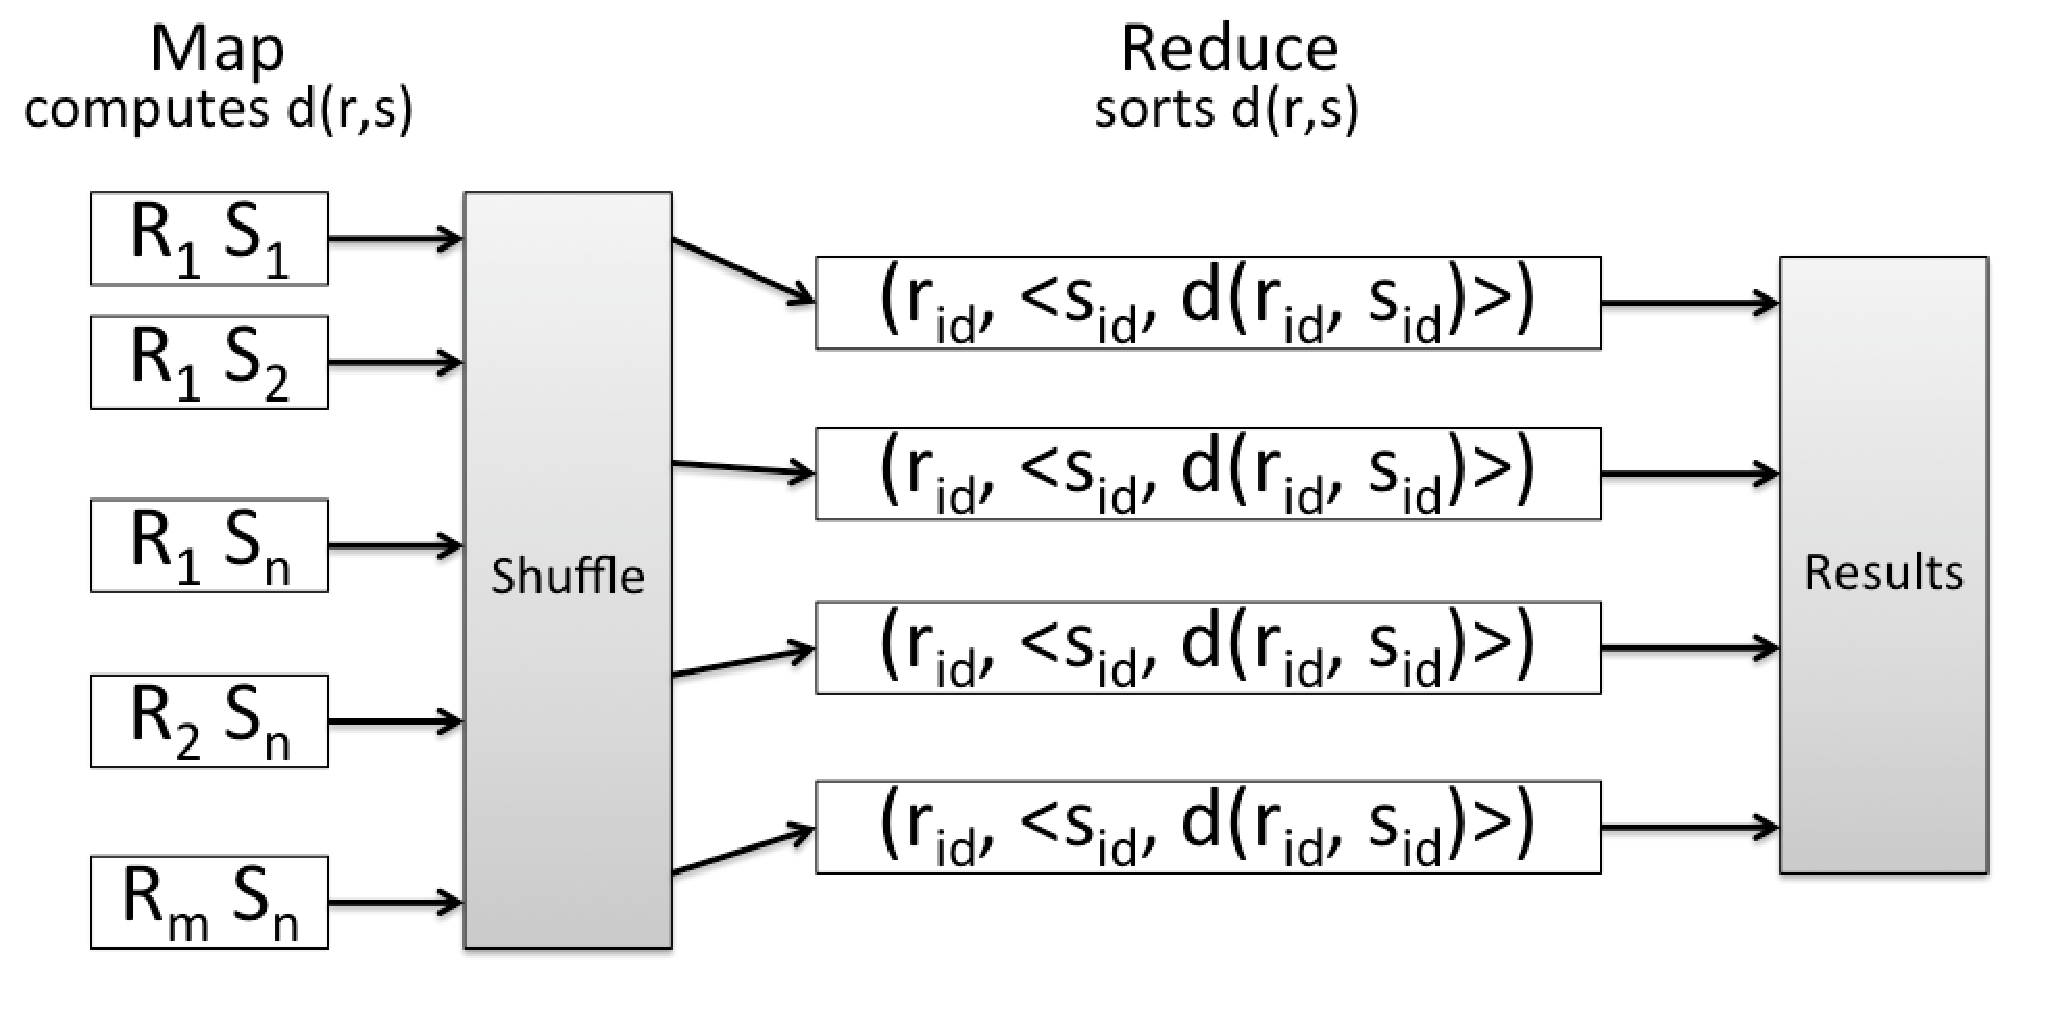
\includegraphics{res/knn-mapreduce.pdf}}
%\caption{Basic idea for processing kNN join in MapReduce \label{knn_mapreduce}}
%\end{figure}
\vspace{0.3em}

\noindent \textbf{With preprocessing and partitioning strategies.} 

\noindent \VO~ \cite{Lu:2012:EPK:2336664.2336674} uses a preprocessing step to select the pivot of each partition and a distance based partitioning 
strategy to ensure that each subset $R_i$ only needs one corresponding subset $S_i$ to form a partition where the kNN of all $r_i \in R_i$ can 
be found. Therefore, in the computation step, Map tasks find the corresponding $S_i$ for each $R_i$ according to the information provided by 
the partitioning step. Reduce tasks then perform the kNN join inside each partition of $<R_i, S_i>$.
%To reduce the number of Map tasks used to calculate the distances, or, in other words, to reduce the number of pairs formed by $R_i$ and $S_j$, PGBJ \cite{Lu:2012:EPK:2336664.2336674} uses a preprocessing and distance based partitioning strategy, which ensures that each partition $R_i$ has only one corresponding partition $S_i$ where the kNN of all $r_i \in R_i$ can be found. This property reduces the number of needed Map tasks to $n$. %In this work, 
%they pre-select similar objects (close points) in $R$ and form a partition with them using distance based partitioning 
%\TODO{not already explained in previous section? --CHECK--}
%, and they subsequently find the 
%corresponding partition in $S$. 
%Once the blocks of $R_i$ and $S_i$ are identified, the same core computation is applied as in the H-BkNNJ technique. 
%Because of 
%their data organization, they are able to reduce the number of tasks, greatly improving the performance.



Overall, the main limitation of these two approaches is that the number of values to be sorted in the Reduce task
can be extremely large, up to $\left|S\right|$, if the
preprocessing and partitioning steps have not significantly reduced the set of searched points.
%when the filtering on the reference points is too coarse. \TODO{reference points? can we say: if the
%pre-processing and partitioning have not significantly reduced the set of candidates}.
%\TODO{I don't like partitioning here, another word like filtering? -- ?? --}. 
This aspect can limit the applicability of such approaches in practice. 


\subsubsection{Two Consecutive MapReduce Jobs}
To overcome the previously described limitation, multiple successive MapReduce jobs are required. The idea is to have the first job output the local top $k$ for each pair $(R_i, S_j)$. Then, the second job is used to merge all the top $k$ values for a given $r_i$ and to merge and sort all local top $k$ values (instead of all values) producing the final global top $k$.

%To overcome the previously described limitation, multiple successive MapReduce jobs are required. The idea is to have the first \emph{job} output
%the local top $k$ for each pair ($R_i$, $S_j$). Then, the second job is used to merge all the top $k$ values for a 
%given $r_i$ and to merge and sort all local top $k$ values (instead of all values), producing the final global top $k$. Such approach is used in H-BNLJ 
%\cite{Zhang:2012:EPK:2247596.2247602} and greatly improves the global performance by reducing sorting time. %And the authors also indicate that we can index the local blocks of S by R-Tree and improve H-BNLJ to H-BRJ.\TODO{is this related to this section?}

%H-BkNNJ method only uses one MapReduce job, but we need to sort $\left|S\right|$ numbers of $d\left(r_i, s_j\right)$ for every object $r_i$. The sort
%algorithm in MapReduce is Quick Sort and Merge Sort by default, their complexity is $\left|S\right| \times Log \left|S\right|$. When $\left|S\right|$ is 
%large, this process is very time consuming. So, paper \cite{Zhang:2012:EPK:2247596.2247602} gives an improvement H-BNLJ. H-BNLJ uses two MapReduce jobs 
%to achieve the same goal. Mapper 1 will get a piece of $R_i$ and $S_j$, Reducer 1 will calculate the distance between $\forall$ $r_i \in R_i$ and $s_j 
%\in S_j$, Mapper 2 sort the results of Reducer 1 and emit the local top $k$ results, Reducer 2 pull the local result of the same key, merge and sort them 
%then give the global top $k$ results. The authors also point out that we can use some index structures like R-Tree to index the local $S$ blocks in order 
%to speed up finding the nearest neighbors.
\vspace{0.3em}

\noindent \textbf{Without preprocessing and partitioning strategies.} 

\noindent \HBNLJ~ does not have any special preprocessing or partitioning strategy. The Map Phase of the first job distributes $R$ into $n$ rows and $S$ into $n$ columns. The $n^2$ Reduce tasks output the local kNN for each object $r_i$ in the form of $(r_{id}, s_{id}, d(r, s))$.

Since each $r_{id}$ has been replicated $n$ times, the Map Phase of the second MapReduce job will pull every candidate of $r_i$ from the $n$ pieces of $R$, and form $(r_{id}), list(s_{id}, d(r, s))$. Then each Reduce task will sort $list(s_{id}, d(r, s))$ in ascending order of $d(r, s)$ for each $r_i$, and finally, give the top $k$ results.

%\TODO{[R2C1] Paper [1]---SOPHIE---Not Checked}
 Moreover, in order to avoid the scan of the whole dataset of each block, some index structures like R-Tree \cite{Zhang:2012:EPK:2247596.2247602} or Hilbert R-Tree \cite{6967143} can be used to index the local $S$ blocks. 

\vspace{0.3em}

\noindent \textbf{With preprocessing and partitioning strategies.} 
%RankReduce  \cite{Stupar10rankreduce-}\footnote{Although RankReduce only compute kNN for a single query, it is 
%directly expandable to a full kNN join} uses LSH to reduce the dimensionality of data in data preprocessing step. Then a size-based partitioning strategy is used to partition the data. So when coming to the computation step, the data is already well partitioned. The Map tasks of the first MapReduce job take one partition of $<R_i, S_i>$, the Reduce tasks will give the local top k results of each $r_i$. And the second MapReduce job will give the global top k results.

\noindent
%the two previous methods: one job for pre-processing and partitioning, one for 
%computing the distances, and a lost one for filtering and sorting the results. 
In \Z~ \cite{Zhang:2012:EPK:2247596.2247602} the authors propose  to define the bounds of the partitions of $R$ and then to determine from this the 
corresponding $S_i$ in a preprocessing job. So here, the preprocessing and partitioning steps are completely integrated in MapReduce. Then, a 
second MapReduce job takes the partitions $R_i$ and $S_i$ previously determined, and computes for all $r_i$ the candidate neighbor set, which 
represents the points that could be in the final kNN\footnote{Note that the notion of candidate points is different from local top $k$ points.}.
To get this candidate neighbor set, the closest $k$ points are taken from either side of the considered point (the partition is in dimension 1), which leads to exactly 2$k$ candidate points.
The third MapReduce round determines the exact result for each $r_i$ from the candidate neighbor set.
%\TODO{how? what does the job do in practice?}
%\TODO{don't like kNN(r,...) here, can it be simpler?}
So in total, this solution uses three MapReduce jobs, and among them, the last two are actually devoted to the kNN core 
computation. As the number of points that are in the candidate neighbor set is small (thanks to the drastic 
partitioning, itself due to a drastic preprocessing), the cost of computation and communication is extremely reduced.

In \LSH~ \cite{Stupar10rankreduce-}\footnote{Although RankReduce only computes kNN for a single query, it is 
directly expandable to a full kNN join.}, the authors first preprocess  data to reduce the dimentionality and partition data into buckets 
using LSH. In our implementation, like in \Z,  one MapReduce job is used to calculate the local kNN for each $r_i$, and 
a second one is used to find the global ones.
